\documentclass[12pt]{beamer}
%\usetheme{Singapore}
\usecolortheme{ietf93color}

\mode<presentation>
\title{IS-IS over IPv6}
\subtitle{%
  \href{https://datatracker.ietf.org/doc/draft-franke-isis-over-ipv6/}{draft-franke-isis-over-ipv6-00}
}
\author{%
	\underline{Christian Franke $\cdot$ \href{mailto:chris@opensourcerouting.org}{chris@opensourcerouting.org}}
}
\date{IETF 93, Prague, Jul. 2015}
\begin{document}

\begin{frame}
  \titlepage
\end{frame}

\begin{frame}
  \frametitle{Motivation}
  \begin{itemize}
    \item \Large Define mode of operation not assuming Ethernet/other specific link-layer
    \item \Large Allow to run IS-IS on any link supporting IPv6
  \end{itemize}
\end{frame}

\begin{frame}
  \frametitle{Structure}
  \begin{itemize}
    \item \Large Keep existing mechanisms and PDU encoding as-is
    \item \Large Specify new transport encapsulation
    \item \Large Specify how new transport should be operated
    \item \Large Clarify consequences of using IS-IS over IPv6
  \end{itemize}
\end{frame}

\begin{frame}
  \frametitle{Packet Format}
  \hspace{13mm}With CLNP:\hspace{32mm}With IS-IS over IPv6:%

  \vspace{5mm}%
    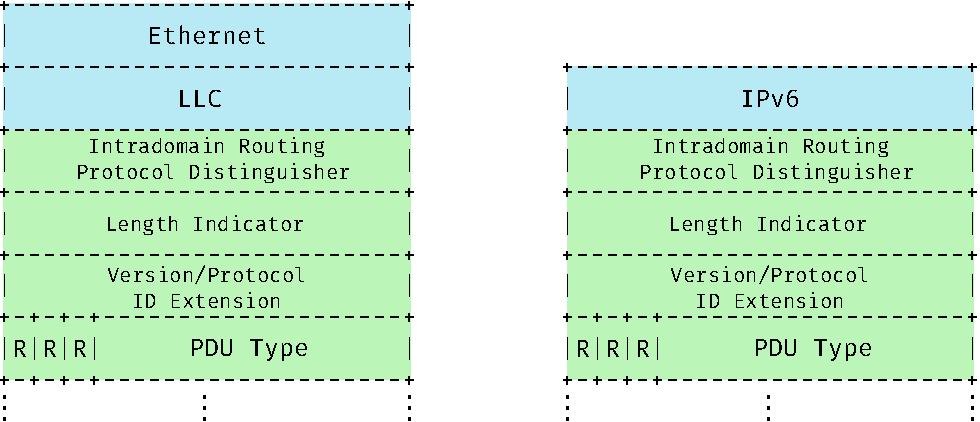
\includegraphics[scale=0.65,angle=0]{isis_ipv6_format-00.pdf}
\end{frame}

\begin{frame}
  \frametitle{Addressing}
  \begin{block}{Packet transmission/reception}
    \begin{itemize}
      \item Routers use IPv6 link-local address as source
      \item Link-local multicast is used as destination
      \begin{itemize}
        \item Multicast group for \texttt{ALL-L1-IS}
        \item Multicast group for \texttt{ALL-L2-IS}
      \end{itemize}
    \end{itemize}
  \end{block}
  \begin{block}{SNPA}
    \begin{itemize}
      \item Use link-local source IP in DIS election
    \end{itemize}
  \end{block}
\end{frame}

\begin{frame}
  \frametitle{Considerations}
  \begin{itemize}
    \item Payload size with same MTU is smaller with IS-IS over IPv6
      \begin{itemize}
        \item LSP fragment size needs to be adjusted
        \item Possibly recommend 1240 bytes
      \end{itemize}
    \item Routers MUST make sure to validate that
          received packets are link-local
  \end{itemize}
\end{frame}

\begin{frame}
  \frametitle{Status}
  \begin{block}{Running Code}
    \begin{itemize}
      \item There are two interoperable implementations
    \end{itemize}
  \end{block}
  \begin{block}{Received Feedback}
    \begin{itemize}
      \item Forbid IPv6 fragmentation
      \begin{itemize}
        \item Pad IIHs to max MTU
        \item Only accept packets which aren't fragmented
        \item Possibly forbid fragmentation only for IIHs?
      \end{itemize}
      \item Use UDP instead
      \begin{itemize}
        \item Allows running multiple IS-IS implementations concurrently on the
              same network
      \end{itemize}
    \end{itemize}
  \end{block}
\end{frame}
\end{document}
